
\caulc 

%%%============= EX_1 =============%%%
\begin{ex}%[1D6H4-3]%[TDMZZ05-1-TN]%[Mui Doan]
	Tập nghiệm của bất phương trình $\log_{0{,}7}(x-2)>0$ là
	\choice
	{$(3;+\infty)$}
	{$(-\infty;3)$}
	{\True $(2;3)$}
	{$(3;4)$}
	\loigiai{
		Điều kiện $x-2>0\Leftrightarrow x>2$.\\
		Ta có $\log_{0{,}7}(x-2)>0\Leftrightarrow x-2<1\Leftrightarrow x<3$.\\
		So điều kiện ta có $x\in (2;3)$.
	}
\end{ex}

%%%============= EX_2 =============%%%
\begin{ex}%[1H8H7-2][TDMZZ07][Huỳnh Trí Thiện]
	\immini[thm]{Cho hình chóp tam giác $S.ABC$ có đáy là tam giác đều cạnh $a$. Cạnh bên $SA$ vuông góc với đáy $(ABC)$ và có $SA=2a$. Thể tích khối chóp $S.ABC$ bằng
		\choice
		{$\dfrac{a^3 \sqrt{3}}{2}$}
		{\True $\dfrac{a^3 \sqrt{3}}{6}$}
		{$\dfrac{a^3 \sqrt{3}}{12}$}
		{$\dfrac{a^3 \sqrt{6}}{12}$}}{	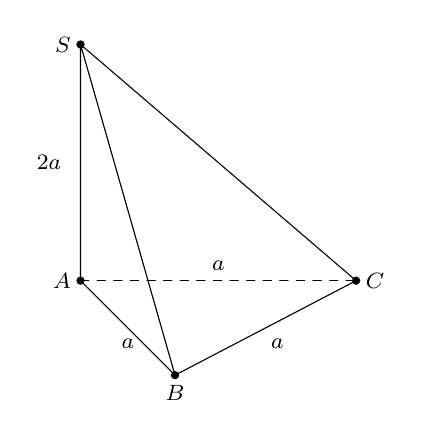
\begin{tikzpicture}[scale=1, font=\footnotesize, line join=round, line cap=round]
			\coordinate (A) at (0,0);
			\coordinate (B) at (1.2,-1.2);
			\coordinate (C) at (3.5,0);
			\coordinate (S) at (0,3);
			
			\draw (S)--(A)--(B)--(C)--cycle (S)--(B) (S)--(C);
			\draw[dashed] (A)--(C);
			
			\fill (A) circle (1.5pt) node[left] {$A$};
			\fill (B) circle (1.5pt) node[below] {$B$};
			\fill (C) circle (1.5pt) node[right] {$C$};
			\fill (S) circle (1.5pt) node[left] {$S$};
			
			\node at (-0.4, 1.5) {$2a$};
			\node at (0.6, -0.8) {$a$};
			\node at (2.5, -0.8) {$a$};
			\node[above] at (1.75, 0) {$a$};
		\end{tikzpicture}
	}
	\loigiai{
		Thể tích khối chóp $S.ABC$ là
		\[ V_{S.ABC} = \dfrac{1}{3} \cdot S_{\triangle ABC} \cdot SA = \dfrac{1}{3} \cdot \dfrac{a^2 \sqrt{3}}{4} \cdot 2a = \dfrac{a^3 \sqrt{3}}{6}. \]
		Vậy thể tích khối chóp bằng $\dfrac{a^3 \sqrt{3}}{6}$.
	}
\end{ex}

%%%============= EX_3 =============%%%
\begin{ex}%[1D2H2-2]%[TDM21]%[Dự án TDM]
	Cho cấp số cộng $(u_n)$ có $u_1 = 1$ và $u_3 = 7$. Công sai của $(u_n)$ bằng
	\choice
	{$6$}
	{$2$}
	{$8$}
	{\True $3$}
	\loigiai{
		Gọi $d$ là công sai của cấp số cộng $(u_n)$.\\
		Theo tính chất của cấp số cộng, ta có
		\begin{align*}
			u_3 &= u_1 + 2d\\
			\Rightarrow 7 &= 1 + 2d\\
			\Rightarrow 2d &= 6\\
			\Rightarrow d &= 3.
		\end{align*}
		Vậy công sai của cấp số cộng đã cho là $d = 3$.
	}
\end{ex}

%%%============= EX_4 =============%%%
\begin{ex}%[1D6V4-5]%[TDMZZ07]%[Dự án TDM]
	Số nghiệm nguyên của bất phương trình $(3+\sqrt{x-4})(3\ln x - \ln^2 x) \ge 0$ là
	\choice
	{$20$}
	{$7$}
	{\True $17$}
	{$4$}
	\loigiai{
		Điều kiện xác định 
		\[ \heva{&x-4 \ge 0\\ &x>0} \Leftrightarrow x \ge 4.\]
		Với mọi $x \ge 4$, ta luôn có $3+\sqrt{x-4} > 0$. Do đó bất phương trình đã cho tương đương với
		\begin{align*}
			3\ln x - \ln^2 x &\ge 0\\
			\Leftrightarrow 0 \le \ln x &\le 3 \\
			\Leftrightarrow \mathrm{e}^0 \le x &\le \mathrm{e}^3 \\
			\Leftrightarrow 1 \le x &\le \mathrm{e}^3.
		\end{align*}
		Kết hợp với điều kiện $x \ge 4$, ta được $4 \le x \le \mathrm{e}^3$.\\
		Vì $x \in \mathbb{Z}$ và $\mathrm{e}^3 \approx 20{,}08$ nên $x \in \{4; 5; 6; \dots; 20\}$.\\
		Vậy bất phương trình đã cho có $17$ nghiệm nguyên.
	}
\end{ex}

%%%============= EX_5 =============%%%
\begin{ex}%[2D4N1-3]%[TDMZZ07]%[Phạm Hải Dương]
	Họ nguyên hàm của hàm số $\dfrac{2}{\sin^2 x}$ với $x \ne k\pi$ ($k \in \mathbb{Z}$), tương ứng là
	\choice
	{$-\tan x + C$}
	{$-\cot x + C$}
	{$-2\tan x + C$}
	{\True $-2\cot x + C$}
	\loigiai{
		Ta có $\displaystyle \int \dfrac{2}{\sin^2 x} \mathrm{\,d}x = 2 \int \dfrac{1}{\sin^2 x} \mathrm{\,d}x = 2(-\cot x) + C = -2\cot x + C$.
	}
\end{ex}

%%%============= EX_6 =============%%%
\begin{ex}%[2D1N2-2]%[TDMZZ03]%[Bồ Văn Hậu]
	\immini[thm]{Cho đồ thị của hàm số $y = f(x)$ như hình vẽ bên. Hỏi hàm số $f(x)$ có tất cả bao nhiêu điểm cực trị?
		\choice
		{\True $4$}
		{$5$}
		{$2$}
		{$3$}}{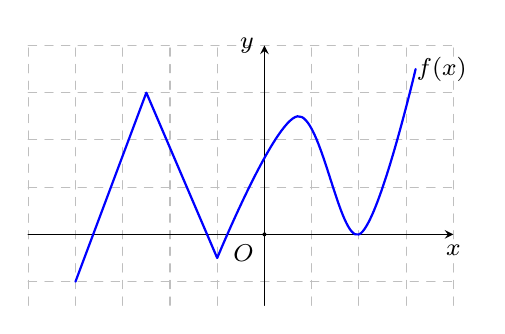
\begin{tikzpicture}[scale=0.6,>=stealth, font=\footnotesize, line join=round, line cap=round]
			\def\xmin{-5} \def\xmax{4}
			\def\ymin{-1.5} \def\ymax{4}
			\tikzset{every node/.style={scale=1.1}}
			\draw[color=gray!50,dashed] (\xmin,\ymin) grid (\xmax,\ymax);
			\draw[->] (\xmin,0)--(\xmax,0) node [below]{$x$};
			\draw[->] (0,\ymin)--(0,\ymax) node [left]{$y$};
			\fill (0,0) circle (1.2pt) node[below left] {$O$};
			\draw[blue,thick] (-4,-1)--(-2.5,3)--(-1,-0.5) plot[smooth,tension=0.6]coordinates { (-1,-0.5) (0.7,2.5) (2,0) (3.2,3.5)};
			\node at (3,3.5) [right]{$f(x)$};
	\end{tikzpicture}}
	\loigiai{
		Dựa vào đồ thị hàm số $y = f(x)$, ta thấy đồ thị có $2$ điểm cực tiểu và có $2$ điểm cực đại.\\
		Vậy hàm số $y = f(x)$ có tất cả $4$ điểm cực trị.
	}
\end{ex}

%%%============= EX_7 =============%%%
\begin{ex}%[2H2H2-4]%[TDMZZ07]%[Nguyễn Sơn Thành]
	Trong không gian với hệ trục tọa độ $Oxyz$, cho hai vectơ $\overrightarrow{u} = (-3;1;-1)$ và $\overrightarrow{v} = (1;0;5)$. Tích vô hướng của hai vectơ này bằng
	\choice
	{\True $-8$}
	{$8$}
	{$3$}
	{$-3$}
	\loigiai{
		Tích vô hướng của hai vectơ $\overrightarrow{u} = (x_1; y_1; z_1)$ và $\overrightarrow{v} = (x_2; y_2; z_2)$ được tính theo công thức
		\[\overrightarrow{u} \cdot \overrightarrow{v} = x_1 \cdot x_2 + y_1 \cdot y_2 + z_1 \cdot z_2.\]
		Áp dụng vào bài toán, ta có
		\[\overrightarrow{u} \cdot \overrightarrow{v} = (-3) \cdot 1 + 1 \cdot 0 + (-1) \cdot 5 = -3 + 0 - 5 = -8.\]
	}
\end{ex}

%%%============= EX_8 =============%%%
\begin{ex}%[2D4H2-1]%[TDMZZ07]%[Lê Phúc]
	Cho biết $\displaystyle\int\limits^1_0 f(x) \mathrm{\,d}x=3$ và $\displaystyle\int\limits^2_1 2f(x) \mathrm{\,d}x=4$. Giá trị của $\displaystyle\int\limits^2_0 f(x) \mathrm{\,d}x$ bằng
	\choice
	{$7$}
	{$12$}
	{\True $5$}
	{$-1$}
	\loigiai{
		Ta có $\displaystyle\int\limits^2_1 2f(x) \mathrm{\,d}x=4\Leftrightarrow \displaystyle\int\limits^2_1 f(x) \mathrm{\,d}x=2$.\\
		Suy ra $\displaystyle\int\limits^2_0 f(x) \mathrm{\,d}x=\displaystyle\int\limits^1_0 f(x) \mathrm{\,d}x+\displaystyle\int\limits^2_1 f(x) \mathrm{\,d}x=3+2=5$.
	}
\end{ex}

%%%============= EX_9 =============%%%
\begin{ex}%[2H5N3-2]%[TDMZZ07]%[Trần Văn Thiện]
	Trong không gian $Oxyz$, cho mặt cầu $(S)\colon x^2+y^2+z^2-4x-2=0$. Bán kính của mặt cầu $(S)$ là
	\choice
	{$6$}
	{$2$}
	{$2\sqrt{2}$}
	{\True $\sqrt{6}$}
	\loigiai{ 
		Mặt cầu $(S)\colon x^2+y^2+z^2-4x-2=0$ có bán kính  $R=\sqrt{2^2-(-2)}=\sqrt{6}$.
	}
\end{ex}

%%%============= EX_10 =============%%%
\begin{ex}%[2D1H3-2]%[TDMZZ07]%[Đình Nguyên]
	Giá trị nhỏ nhất của hàm số $f(x)=x^3-6x$ trên $(0;+\infty)$ bằng
	\choice
	{$0$}
	{$4\sqrt{2}$}
	{\True $-4\sqrt{2}$}
	{$-2\sqrt{2}$}
	\loigiai{
		Xét hàm số $f(x)=x^3-6x$ trên khoảng $(0;+\infty)$.\\
		Ta có $f'(x)=3x^2-6$. \\
		Cho $f'(x)=0 \Leftrightarrow 3x^2-6=0 \Leftrightarrow x^2=2 \Leftrightarrow x=\sqrt{2}$ (vì $x>0$).\\
		Ta có bảng biến thiên
		\begin{center}
			
\begin{tikzpicture}
				\tkzTabInit[nocadre=false, lgt=1.2, espcl=2.5, deltacl=0.6]
				{$x$ /0.6, $f'(x)$ /0.6, $f(x)$ /2}
				{$0$, $\sqrt{2}$, $+\infty$}
				\tkzTabLine{ , -, 0, +, }
				\tkzTabVar{+/ $0$, -/ $-4\sqrt{2}$, +/ $+\infty$}
			\end{tikzpicture}
		\end{center}
		Dựa vào bảng biến thiên, ta thấy $\min\limits_{(0;+\infty)} f(x)=f\left(\sqrt{2}\right)=-4\sqrt{2}$. 
	}
\end{ex}

%%%============= EX_11 =============%%%
\begin{ex}%[1D5V1-3]%[TDMZZ07]%[Huynh Quốc Đạt]
	Cho hai mẫu số liệu nhóm $M_1$, $M_2$ với bảng tần số ghép nhóm
	\begin{center}
		\textbf{\textit{Nhóm $M_1$}} \begin{tabular}{|c|c|c|c|c|c|c|}
			\hline
			\textbf{Nhóm} & $[8;10)$ & $[10;12)$ & $[12;14)$ & $[14;16)$ & $[16;18)$ & $[18;20)$ \\
			\hline
			\textbf{Tần số} & $6$ & $6$ & $8$ & $4$ & $6$ & $7$ \\
			\hline
		\end{tabular}\\
		\vspace{1cm}
		\textbf{\textit{Nhóm $M_2$}} \begin{tabular}{|c|c|c|c|c|c|c|}
			\hline
			\textbf{Nhóm} & $[8;10)$ & $[10;12)$ & $[12;14)$ & $[14;16)$ & $[16;18)$ & $[18;20)$ \\
			\hline
			\textbf{Tần số} & $6$ & $6$ & $8$ & $4$ & $6$ & $a$ \\
			\hline
		\end{tabular}
	\end{center}
	Hỏi có tất cả bao nhiêu giá trị nguyên nhỏ hơn $20$ của $a$ để số trung bình cộng của mẫu số liệu $M_2$ lớn hơn của mẫu số liệu $M_1$?
	\choice
	{$11$}
	{\True $12$}
	{$13$}
	{$6$}
	\loigiai{Ta có bảng giá trị đại diện của hai nhóm
		\begin{center}
			\textbf{\textit{Nhóm $M_1$}} \begin{tabular}{|c|c|c|c|c|c|c|}
				\hline
				\textbf{Nhóm} & $[8;10)$ & $[10;12)$ & $[12;14)$ & $[14;16)$ & $[16;18)$ & $[18;20)$ \\
				\hline
				\textbf{Giá trị đại diện} & $9$ &$11$ & $13$ & $15$ & $17$ & $19$\\
				\hline
				\textbf{Tần số} & $6$ & $6$ & $8$ & $4$ & $6$ & $7$ \\
				\hline
			\end{tabular}\\
			\vspace{1cm}
			\textbf{\textit{Nhóm $M_2$}} \begin{tabular}{|c|c|c|c|c|c|c|}
				\hline
				\textbf{Nhóm} & $[8;10)$ & $[10;12)$ & $[12;14)$ & $[14;16)$ & $[16;18)$ & $[18;20)$ \\
				\hline
				\textbf{Giá trị đại diện} & $9$ &$11$ & $13$ & $15$ & $17$ & $19$\\
				\hline
				\textbf{Tần số} & $6$ & $6$ & $8$ & $4$ & $6$ & $a$ \\
				\hline
			\end{tabular}
		\end{center}
		\begin{itemize}
			\item Nhóm $M_1$:\\
			Ta có cỡ mẫu $N_1=6+6+8+4+6+7=37$.\\
			Số trung bình của nhóm $M_1$ là \[\overline{x}_1=\dfrac{54+66+104+60+102+133}{37}=\dfrac{519}{37}.\]
			\item Nhóm $M_2$:\\
			Ta có cỡ mẫu $N_2=6+6+8+4+6+a=30+a$.\\
			Số trung bình của nhóm $M_2$ là \[\overline{x}_2=\dfrac{54+66+104+60+102+19a}{30+a}=\dfrac{386+19a}{30+a}.\]
		\end{itemize}
		Vì $\overline{x}_2 > \overline{x}_1$ nên
		\begin{align*}
			\dfrac{386+19a}{30+a} &> \dfrac{519}{37}\\
			\Leftrightarrow 37(386+19a) &> 519(30+a)\\
			\Leftrightarrow 14\,282 + 703a &> 15\,570 + 519a\\
			\Leftrightarrow 184a &> 1\,288\\
			\Leftrightarrow a &> 7.
		\end{align*}
		Mà $a$ nguyên và $a < 20$ nên $a \in \{8; 9; 10; \dots; 19\}$.\\
		Vậy có tất cả $12$ giá trị $a$ thoả mãn yêu cầu bài toán.
	}
\end{ex}

%%%============= EX_12 =============%%%
\begin{ex}%[2H2H2-4]%[TDMZZ07]%[Nguyễn Trí Minh Tuấn]
	Cho tứ diện đều $ABCD$ có cạnh bằng $6$. Giá trị 
	$\left(\overrightarrow{AB}+\overrightarrow{AC}\right)\cdot \overrightarrow{AD}$
	bằng
	\choice
	{\True $36$}
	{$0$}
	{$18\sqrt{3}$}
	{$72$}
	\loigiai{
		\immini{Vì $ABCD$ là tứ diện đều nên các mặt $ABD$ và $ACD$ đều là tam giác đều cạnh $6$. \\
			Do đó $AB=AC=AD=6$, $\widehat{BAD}=\widehat{CAD}=60^\circ$.\\
			Suy ra
			\begin{align*}
				\left(\overrightarrow{AB}+\overrightarrow{AC}\right)\cdot \overrightarrow{AD}
				&= \overrightarrow{AB}\cdot \overrightarrow{AD} + \overrightarrow{AC}\cdot \overrightarrow{AD}\\
				&= AB\cdot AD\cdot \cos \widehat{BAD} + AC\cdot AD\cdot \cos \widehat{CAD}\\
				&= 6\cdot 6\cdot \cos 60^\circ + 6\cdot 6\cdot \cos 60^\circ\\
				&= 36\cdot \dfrac{1}{2} + 36\cdot \dfrac{1}{2}\\
				&= 36.
			\end{align*}
		}{
			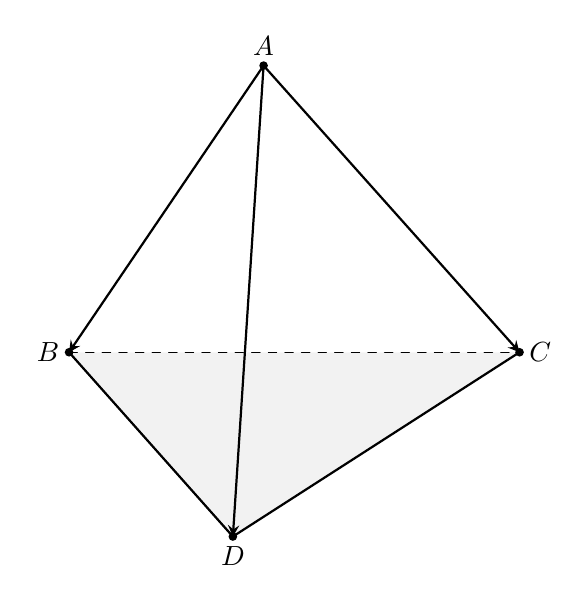
\begin{tikzpicture}[scale=1.3, line join=round, line cap=round, >=stealth]
				% Tọa độ
				\coordinate (B) at (0,0);
				\coordinate (C) at (4.4,0);
				\coordinate (D) at (1.6,-1.8);
				\coordinate (A) at (1.9,2.8);
				
				% Mặt đáy
				\fill[gray!10] (B)--(C)--(D)--cycle;
				
				% Cạnh khuất
				\draw[dashed] (B)--(C);
				
				% Các cạnh nhìn thấy
				\draw[thick] (B)--(D)--(C);
				\draw[thick,->] (A)--(B);
				\draw[thick,->] (A)--(C);
				\draw[thick,->] (A)--(D);
				
				% Điểm
				\fill (A) circle (1.2pt) node[above] {$A$};
				\fill (B) circle (1.2pt) node[left] {$B$};
				\fill (C) circle (1.2pt) node[right] {$C$};
				\fill (D) circle (1.2pt) node[below] {$D$};
			\end{tikzpicture}
		}
	}
\end{ex}
\cauds

%%%============= EX_13 =============%%%
\begin{ex}%[2D4H3-1]%[Dương Công Tạo]
	Cho hàm số $y = f(x) = \dfrac{x^2 + ax + b}{x-1}$ có đồ thị $(C)$, có tâm đối xứng là điểm $I(1;3)$ và cắt trục tung tại điểm có tung độ bằng $4$.
	\choiceTF
	{\True $(2;2)\in(C)$}
	{$a+b=2$}
	{Đường thẳng đi qua hai điểm cực trị của $(C)$ là $y = 2x +1$}
	{\True Diện tích hình phẳng giới hạn bởi $(C)$, trục hoành, đường thẳng $y = 2$ bằng $7$ (\textit{làm tròn kết quả đến hàng đơn vị})}
	\loigiai{
		Với mọi $x\ne 1$, hàm số được viết lại $y=f(x)=x+a+1+\dfrac{a+b+1}{x-1}$.\\
		Với mọi $x\ne 1$ và $a+b+1\ne 0$, đồ thị hàm số đã cho nhận
		\begin{itemize}
			\item đường thẳng $x=1$ làm tiệm cận đứng.
			\item đường thẳng $y=x+a+1$ làm tiệm cận xiên.
		\end{itemize}
		Khi đó, để đồ thị $(C)$ nhận điểm $I(1;3)$ là tâm đối xứng thì 
		\[\heva{&a+b+1\ne 0\\&1+a+1=3}\Leftrightarrow\heva{&a=1\\&b\ne-2.}\]
		Mặt khác, vì đồ thị $(C)$ cắt trục tung tại điểm có tung độ bằng $4$ nên 
		\[(0;4)\in(C)\Leftrightarrow \dfrac{b}{-1}=4 \Leftrightarrow b=-4.\]
		Vậy $(C)\colon y=f(x)=\dfrac{x^2+x-4}{x-1}$.
		\begin{itemchoice}
			\itemch Thế toạ độ điểm $(2;2)$ vào $(C)$ ta được $\dfrac{2^2+2-4}{2-1}=2$ (đúng).\\
			Do đó, $(2;2)\in(C)$.
			\itemch Ta có $a=1$, $b=-4$. Suy ra $a+b=-3$.
			\itemch Với $x\ne 1$, ta có $f'(x)=\dfrac{x^2-2x+3}{(x-1)^2}=\dfrac{(x-1)^2+2}{(x-1)^2}>0$, $\forall x\ne 1$.\\
			Suy ra hàm số đã cho luôn đồng biến trên từng khoảng xác định và không đạt cực trị.
			\itemch Xét phương trình hoành độ theo biến $y$:
			\[ y = \dfrac{x^2+x-4}{x-1} \Leftrightarrow x^2 + (1-y)x + y - 4 = 0. \]
			Với $y \in [0; 2]$, ta có $\Delta = (1-y)^2 - 4(y-4) = y^2 - 6y + 17 > 0$.\\
			Phương trình luôn có hai nghiệm phân biệt (tương ứng với hai nhánh của đồ thị $(C)$):
			\[ x_1 = \dfrac{y-1 - \sqrt{y^2-6y+17}}{2}; \quad x_2 = \dfrac{y-1 + \sqrt{y^2-6y+17}}{2} \quad (x_1 < x_2). \]
			Diện tích hình phẳng giới hạn bởi đồ thị $(C)$, trục hoành ($y=0$) và đường thẳng $y=2$ là diện tích miền kín nằm giữa hai nhánh của đồ thị.\\
			Áp dụng công thức tính diện tích theo biến $y$, ta có:
			\[ S = \displaystyle\int\limits_0^2 (x_2 - x_1) \mathrm{\,d}y = \displaystyle\int\limits_0^2 \sqrt{y^2-6y+17} \mathrm{\,d}y. \]
			Sử dụng máy tính cầm tay, ta tính được $S \approx 6{,}993$.\\
			Làm tròn kết quả đến hàng đơn vị, ta được $S \approx 7$. 
		\end{itemchoice}
	}
\end{ex}

%%%============= EX_14 =============%%%
\begin{ex} %[TDMZZ07]%[Hà Văn Hảo]%[2D4C2-6]
	Một vật bắt đầu chuyển động thẳng từ địa điểm $A$ đến dừng lại tại địa điểm $B$ (cách $A$ một khoảng bằng $1\,500$ mét). Biết vật chuyển động với vận tốc $v(t) = \heva{&at + b && 0 \le t < 30 \\ &24 && 30 \le t \le 60 \\ &mt^2 + n && 60 \le t \le t_2 }$ (m/s). Trong đó thời gian $t$ tính theo giây, gốc thời gian tính từ $A$. 
	\choiceTF
	{\True $a = 0{,}8$; $b = 0$}
	{\True Quãng đường vật đi được trong $30$ giây đầu là $360$ m (\textit{làm tròn kết quả đến hàng đơn vị})}
	{\True Quãng đường vật chuyển động chậm dần (giảm tốc) là $420$ m}
	{Tổng thời gian để vật đi từ $A$ đến $B$ bằng $120$ giây (\textit{làm tròn kết quả đến hàng đơn vị khi tính theo giây})}
	\loigiai{
		\begin{itemchoice}
			\itemch Tại thời điểm $t = 0$, vật bắt đầu chuyển động nên $v(0) = 0 \Rightarrow a \cdot 0 + b = 0 \Rightarrow b = 0$.\\
			Tại thời điểm $t = 30$, do tính liên tục của vận tốc, ta có $a \cdot 30 + b = 24 \Rightarrow a = 0{,}8$.\\
			Vậy $a = 0{,}8$ và $b = 0$. 
			\itemch Quãng đường vật đi được trong $30$ giây đầu là
			\[s_1 = \displaystyle\int\limits_0^{30} 0{,}8t \mathrm{\,d}t = \left. 0{,}4t^2 \right|_0^{30} = 0{,}4 \cdot 30^2 = 360\text{ (m).}\]
			\itemch Quãng đường vật đi được trong giai đoạn vận tốc không đổi ($30 \le t \le 60$) là
			\[s_2 = 24 \cdot (60 - 30) = 720\text{ (m).}\]
			Tổng quãng đường đi được trong hai giai đoạn đầu là $s_1 + s_2 = 360 + 720 = 1\,080\text{ (m)}$.\\
			Quãng đường vật chuyển động chậm dần (giai đoạn $3$) là
			\[s_3 = AB - \left(s_1 + s_2\right) = 1\,500 - 1\,080 = 420\text{ (m).}\]
			\itemch Trong giai đoạn $3$ ($60 \le t \le t_2$).\\
			Tại $t = 60$ thì $v(60) = 24 \Leftrightarrow m \cdot 60^2 + n = 24 \Leftrightarrow 3\,600m + n = 24$.\\
			Tại $t = t_2$, vật dừng lại nên $v(t_2) = 0 \Leftrightarrow mt_2^2 + n = 0 \Leftrightarrow n = -mt_2^2$.\\
			Thay vào phương trình trên $m(3\,600 - t_2^2) = 24 \Rightarrow m = \dfrac{24}{3\,600 - t_2^2}$.\\
			Quãng đường giai đoạn $3$ là
			\[s_3 = \displaystyle\int\limits_{60}^{t_2} (mt^2 + n)\mathrm{\,d}t = \left. \left( \dfrac{mt^3}{3} + nt \right) \right|_{60}^{t_2} = m \left( \dfrac{t_2^3 - 60^3}{3} \right) + n(t_2 - 60) = 420.\]
			Thay $n = -mt_2^2$ và $m = \dfrac{24}{3\,600 - t_2^2}$, ta được
			\begin{align*}
				& m \left[ \dfrac{t_2^3 - 216\,000}{3} - t_2^2\left(t_2 - 60\right) \right] = 420\\
				\Leftrightarrow \quad & m \left( \dfrac{t_2^3 - 216\,000 - 3t_2^3 + 180t_2^2}{3} \right) = 420\\
				\Leftrightarrow \quad & \dfrac{24}{3\,600 - t_2^2} \cdot \dfrac{-2t_2^3 + 180t_2^2 - 216\,000}{3} = 420\\
				\Leftrightarrow \quad & 8 \cdot \dfrac{-2\left( t_2^3 - 90t_2^2 + 108\,000 \right)}{-\left(t_2^2 - 3\,600\right)} = 420 \\
				\Leftrightarrow \quad & \dfrac{16\left( t_2 - 60 \right)^2\left( t_2 + 30 \right)}{\left( t_2 - 60 \right)\left( t_2 + 60 \right)} = 420\\
				\Leftrightarrow \quad & \dfrac{16\left( t_2 - 60 \right)\left( t_2 + 30 \right)}{t_2 + 60} = 420 \\
				\Leftrightarrow \quad & 16\left( t_2^2 - 30t_2 - 1\,800 \right) = 420t_2 + 25\,200\\
				\Leftrightarrow \quad & 16t_2^2 - 480t_2 - 28\,800 = 420t_2 + 25\,200 \\
				\Leftrightarrow \quad & 16t_2^2 - 900t_2 - 54\,000 = 0\\
				\Leftrightarrow \quad & \hoac{&t_2 = \dfrac{225 + 75\sqrt{47}}{8} \approx 92{,}67 \text{ (nhận)}\\ &t_2 = \dfrac{225 - 75\sqrt{47}}{8} \approx -36{,}42 \text{ (loại)}.}
			\end{align*}
			Làm tròn kết quả đến hàng đơn vị, tổng thời gian để vật đi từ $A$ đến $B$ bằng $93$ giây.
		\end{itemchoice}
	}
\end{ex}

%%%============= EX_15 =============%%%
\begin{ex}%[2D6V2-4]%[TDMZZ05]%[Vũ Hồng Toàn]
	Một thống kê cho thấy tỉ lệ dân số mắc bệnh hiểm nghèo $X$ là $0{,}4\%$. Bác Hải đi xét nghiệm bệnh hiểm nghèo $X$ và nhận được kết quả âm tính. Biết rằng, nếu thật sự mắc bệnh hiểm nghèo $X$ thì sẽ cho $7\%$ xét nghiệm chẩn đoán sai, nếu không mắc bệnh hiểm nghèo $X$ thì sẽ cho $4\%$ xét nghiệm chẩn đoán sai. Gọi $A$ là biến cố bác Hải nhận được kết quả âm tính, $B$ là biến cố bác Hải thật sự mắc bệnh hiểm nghèo $X$.
	\choiceTF
	{\True Trước khi đi xét nghiệm xác suất bác Hải không mắc bệnh $X$ là $0{,}996$}
	{\True $\mathrm{P}\left(A\mid B\right) = \dfrac{7}{100}$}
	{$\mathrm{P}\left(A\right) = 0{,}93$ (\textit{làm tròn kết quả đến hàng phần trăm})}
	{\True Sau khi xét nghiệm cho kết quả âm tính, xác suất để bác Hải không mắc bệnh $X$ là $0{,}99971$}
	\loigiai{
		Ta có
		\begin{itemize}
			\item Xác suất mắc bệnh là $\mathrm{P}\left(B\right) = 0{,}4\% = 0{,}004$.
			\item Xác suất không mắc bệnh là $\mathrm{P}\left(\overline{B}\right) = 1 - \mathrm{P}\left(B\right) = 1 - 0{,}004 = 0{,}996$.
			\item Nếu mắc bệnh ($B$), xác suất chẩn đoán sai (tức là kết quả âm tính $A$) là $\mathrm{P}\left(A\mid B\right) = 7\% = 0{,}07$.
			\item Nếu không mắc bệnh ($\overline{B}$), xác suất chẩn đoán sai (tức là kết quả dương tính $\overline{A}$) là $\mathrm{P}\left(\overline{A}\mid \overline{B}\right) = 4\% = 0{,}04$.
			\item Suy ra, nếu không mắc bệnh ($\overline{B}$), xác suất chẩn đoán đúng (tức là kết quả âm tính $A$) là $\mathrm{P}\left(A\mid \overline{B}\right) = 1 - \mathrm{P}\left(\overline{A}\mid \overline{B}\right) = 1 - 0{,}04 = 0{,}96$.
		\end{itemize}
		\begin{itemchoice}
			\itemch Xác suất bác Hải không mắc bệnh trước khi xét nghiệm là $\mathrm{P}\left(\overline{B}\right) = 0{,}996$.
			\itemch $\mathrm{P}\left(A\mid B\right) = 0{,}07 = \dfrac{7}{100}$.
			\itemch Xác suất để bác Hải nhận kết quả âm tính là
			\[\mathrm{P}\left(A\right) = \mathrm{P}\left(B\right) \cdot \mathrm{P}\left(A\mid B\right) + \mathrm{P}\left(\overline{B}\right) \cdot \mathrm{P}\left(A\mid\overline{B}\right) = 0{,}004 \cdot 0{,}07 + 0{,}996 \cdot 0{,}96 = 0{,}95644 \approx 0{,}96 \ne 0{,}93.\]
			\itemch Xác suất bác Hải không mắc bệnh khi đã biết kết quả âm tính là:
			\[\mathrm{P}\left(\overline{B}\mid A\right) = \dfrac{\mathrm{P}\left(\overline{B}\right) \cdot \mathrm{P}\left(A\mid\overline{B}\right)}{\mathrm{P}\left(A\right)} = \dfrac{0{,}996 \cdot 0{,}96}{0{,}95644}  \approx 0{,}99971.\]
		\end{itemchoice}
	}
\end{ex}

%%%============= EX_16 =============%%%
\begin{ex}%[2H5V3-4]%[TDMZZ07]%[Văn Minh Thoại]
	\immini[thm]{
		Trong không gian $Oxyz$, coi Trái Đất là một hình cầu có tâm là gốc toạ độ và có bán kính bằng $16$, đơn vị dài trên mỗi trục toạ độ là $400$ km. Coi tầng điện ly luôn cách bề mặt Trái Đất $400$ km, tức là tầng điện ly là một mặt cầu có tâm là gốc toạ độ $O$. Từ một đài phát $A$ đặt tại điểm $A(16;0;0)$ có phát một sóng điện từ với tần số $10$ MHz lên trên cao (với tốc độ không đổi bằng $3\cdot 10^8$ m/s) hướng theo vectơ $\overrightarrow{u}=(1;2;0)$, sóng điện từ này gặp tầng điện ly tại điểm $B$, tại $B$ nó bị phản xạ và truyền trở lại gặp bề mặt Trái Đất tại điểm $C$. Biết rằng tính chất phản xạ cho ta kết quả là bốn điểm $O$, $A$, $B$, $C$ đồng phẳng và có $\widehat{ABO}=\widehat{OBC}$, $\widehat{AOB}=\widehat{BOC}$.
	}{
		\begin{tikzpicture}[>=stealth,scale=0.8, line join=round,line cap=round,every node/.style={font=\footnotesize},declare function={R1 = 2.5; R2 = 4; goca =15; gocb=48; gocc = 80;}]
			\path (0,0) coordinate (O)
			(goca:R1) coordinate (A)
			(gocb:R2) coordinate (B)
			(gocc:R1) coordinate (C);
			\draw[fill=cyan!30!yellow] (O) circle (R1);
			\node at (-90:R1*0.45) {\textbf{\textit{Trái Đất}}};
			\draw[color=red!80!black,line width=0.6pt] (O) circle (R2);
			\node at (25:R2*1.3) {Tầng điện ly};
			\draw (O) -- (A) -- (B) -- (C);
			\draw[->] (A) -- ($(A)!0.7cm!(B)$) node[right=-1pt] {$\overrightarrow{u}$};
			\draw[fill=red] (O) circle (1pt) node[shift={(-45:10pt)}] {$O$};
			\draw[fill=red] (A) circle (1pt) node[shift={(0:10pt)}] {$A$};
			\draw[fill=red] (B) circle (1pt);
			\draw[fill=red] (C) circle (1pt);
			\node[above left=5pt] at (A) {$AC = 1\,361$ km};
			\node[above right=-2pt] at (B) {$B$};
			\node[above left=-2pt] at (C) {$C$};
		\end{tikzpicture}
	}
	\choiceTF
	{\True Tầng điện ly là mặt cầu có tâm $O(0;0;0)$ và bán kính bằng $17$}
	{\True Phương trình tham số của đường thẳng $AB$ là $\heva{&x=16+t\\&y=2t\\&z=0}$}
	{Nếu toạ độ điểm $B$ là $(a;b;c)$ thì $(a+2b+c)^2=256$}
	{\True Tính theo đơn vị km \textit{(làm tròn đến hàng đơn vị)} thì ta có $AC=1\,361$ km}
	\loigiai{
		\begin{itemchoice}
			\itemch Vì tầng điện ly cách bề mặt Trái Đất $400$ km (tương ứng với $1$ đơn vị dài) nên bán kính mặt cầu tầng điện ly là $R'=16+1=17$. \\
			Tâm của mặt cầu này là $O(0;0;0)$.
			\itemch Đường thẳng $AB$ đi qua đài phát $A(16;0;0)$ và có vectơ chỉ phương $\overrightarrow{u}=(1;2;0)$ nên có phương trình tham số là $\heva{&x=16+t\\&y=2t\\&z=0.}$
			\itemch Toạ độ điểm $B$ là giao điểm của tia $AB$ ($t>0$) và mặt cầu tầng điện ly có phương trình $x^2+y^2+z^2=17^2=289$.
			Thay phương trình tham số $AB$ vào mặt cầu, ta được
			\begin{align*}
				&(16+t)^2+(2t)^2+0^2=289\\
				\Leftrightarrow \quad &256+32t+t^2+4t^2=289\\
				\Leftrightarrow \quad &5t^2+32t-33=0\\
				\Leftrightarrow \quad &\hoac{&t=\dfrac{-16+\sqrt{421}}{5}&\text{(nhận)}\\&t=\dfrac{-16-\sqrt{421}}{5}&\text{(loại)}.}
			\end{align*}
			Vì $B\in AB$ suy ra $B(16+t;2t;0)$ hay $B\left(\dfrac{64+\sqrt{421}}{5};\dfrac{-32+2\sqrt{421}}{5};0\right)$.\\
			Ta có toạ độ $B(a;b;c)$ nên $a=\dfrac{64+\sqrt{421}}{5}$, $b=\dfrac{-32+2\sqrt{421}}{5}$, $c=0$.\\
			Khi đó
			\[(a+2b+c)^2=\left(\dfrac{64+\sqrt{421}}{5}+2\cdot \dfrac{-32+2\sqrt{421}}{5}+0\right)^2=421\ne 256.\]
			\immini{\itemch
				Đặt $\alpha=\widehat{AOB}$. \\
				Ta có
				\begin{align*}
					&\overrightarrow{OA}\cdot\overrightarrow{OB}=OA\cdot OB\cdot\cos\alpha\\
					\Leftrightarrow \quad &16(16+t)+0+0=16\cdot 17\cdot\cos\alpha\\
					\Leftrightarrow \quad &\cos\alpha=\dfrac{16+t}{17}.
				\end{align*}
				Thay giá trị của $t$ vào, ta được \[\cos\alpha=\dfrac{16+\dfrac{-16+\sqrt{421}}{5}}{17}=\dfrac{64+\sqrt{421}}{85}.\]
				Theo giả thiết $\triangle OAB=\triangle OCB$ (c.g.c) nên $\widehat{AOC}=2\alpha$.
			}{
				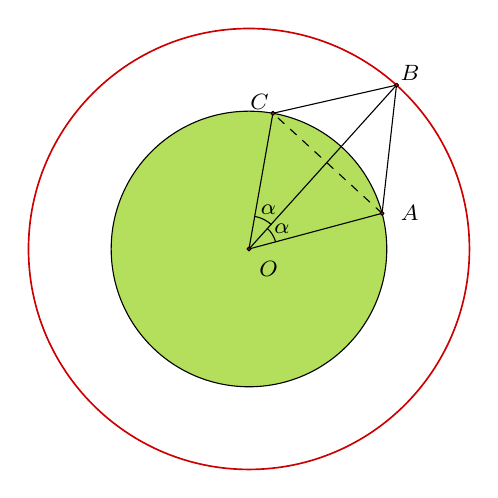
\begin{tikzpicture}[>=stealth,scale=0.7, line join=round,line cap=round,every node/.style={font=\footnotesize},declare function={R1 = 2.5; R2 = 4; goca =15; gocb=48; gocc = 80;}]
					\path (0,0) coordinate (O)
					(goca:R1) coordinate (A)
					(gocb:R2) coordinate (B)
					(gocc:R1) coordinate (C);
					\draw[fill=cyan!30!yellow] (O) circle (R1);
					\draw[color=red!80!black,line width=0.6pt] (O) circle (R2);
					\draw (A) -- (O) -- (C);
					\draw (O) -- (B);
					\draw (A) -- (B) -- (C);
					\draw[dashed] (A) -- (C);
					\draw[fill=red] (O) circle (1pt) node[shift={(-45:10pt)}] {$O$};
					\draw[fill=red] (A) circle (1pt) node[shift={(0:10pt)}] {$A$};
					\draw[fill=red] (B) circle (1pt) node[above right=-2pt] {$B$};
					\draw[fill=red] (C) circle (1pt) node[above left=-2pt] {$C$};
					% draw angles
					\draw (O) ++(goca:0.5) arc (goca:gocb:0.5);
					\node at (31.5:0.7) {$\alpha$};
					\draw (O) ++(gocb:0.6) arc (gocb:gocc:0.6);
					\node at (64:0.8) {$\alpha$};
				\end{tikzpicture}
			}
			\noindent Trong $\triangle OAC$ cân tại $O$, ta có
			\begin{align*}
				AC^2 &= OA^2+OC^2-2\cdot OA\cdot OC\cdot\cos(2\alpha)\\
				&= 2\cdot 16^2-2\cdot 16^2\cdot\left(2\cos^2\alpha-1\right)\\
				&= 1\,024\cdot\left(1-\cos^2\alpha\right)\\
				&= 1\,024\sin^2\alpha.
			\end{align*}
			Suy ra $AC=32\sin\alpha=32\sqrt{1-\cos^2\alpha}$.\\
			Thay giá trị chính xác của $\cos\alpha$, ta tính được
			\[ AC = 32\sqrt{1-\left(\dfrac{64+\sqrt{421}}{85}\right)^2} \approx 3{,}4029 \text{ (đơn vị dài).}\]
			Vì đơn vị dài trên mỗi trục toạ độ là $400$ km nên $AC\approx 3{,}4029\cdot 400\approx 1\,361$ km.
		\end{itemchoice}
	}
\end{ex}


\caukq

%%%============= EX_17 =============%%%
\begin{ex}%[1H8V5-4]%[TDMZZ07]%[Võ Hiệp]
	Cho hình lăng trụ $ABCD.A'B'C'D'$ có đáy $ABCD$ là hình bình hành. Gọi $H$ là hình chiếu vuông góc của $A$ trên đáy $(A'B'C'D')$. Biết $H$ cách đều hai cạnh $A'B'$, $C'D'$ một khoảng bằng $4$, có $AH = 6$. Hãy tính khoảng cách giữa hai đường thẳng $AA'$ và $C'D'$ ({\it làm tròn kết quả đến hàng phần trăm}).
	\par\shortans[]{$6{,}66$}
	\loigiai{
		\immini{
			Hình lăng trụ $ABCD.A'B'C'D'$ có đáy $ABCD$ là hình bình hành.
			Suy ra $A'B'\parallel C'D'$.\\
			Trong mặt phẳng $(A'B'C'D')$ kẻ đường thẳng $d$ đi qua $H$ vuông góc và cắt $A'B'$, $C'D'$ lần lượt tại $M$ và $N$.\\
			Ta có $\heva{&A'B'\subset (A'B'C'D')\\& A'B'\parallel C'D'}\Rightarrow C'D'\parallel (A'B'C'D')$.\\
			Mà $AA'\subset (A'B'C'D')$, $N\in (C'D')$. Do đó\\
			$\mathrm{d}(AA',C'D')=\mathrm{d}\big(C'D',(A'B'C'D')\big)=\mathrm{d}\big(N,(A'B'C'D')\big)$.\\
			Kẻ $HI\perp AM$ tại $I$.
		}{
			\begin{tikzpicture}[scale=1,>=stealth, font=\footnotesize, line join=round, line cap=round]
				\def\a{3.5}
				\def\h{4}
				\path 	(0:0) coordinate (A')
				++(0:\a) coordinate (D')
				++(-130:\a/2) coordinate (C')
				($(A')+(C')-(D')$) coordinate (B')
				($(A')!.4!(B')$) coordinate (M)	
				($(C')!.2!(D')$) coordinate (N)	
				($(M)!0.5!(N)$) coordinate (H)
				($(H)+(90:\h)$) coordinate (A)
				($(A)+(C')-(A')$) coordinate (C)
				($(C)+(B')-(C')$) coordinate (B)
				($(A)+(D')-(A')$) coordinate (D)
				($(A)!.75!(M)$) coordinate (I)	;
				\draw[dashed] 	(B')--(A')--(D')	(A)--(A') (A)--(H) (A)--(M)--(H)--(N) (H)--(I);
				\draw (C)--(C') 	(D)--(D') 	(B)--(B')  (B')--(C')--(D') (A)--(B)--(C)--(D)--cycle;
				\foreach \x/\g in {A/150,B/-150,C/-30,D/30,A'/-70,B'/-150,C'/-30,D'/-30,H/-135,M/-60,N/-30,I/120}
				\fill[black] 	(\x) circle (1pt)
				($(\g:3mm)+(\x)$) node {$\x$};
				\draw pic[draw,angle radius=1.5mm]{right angle=H--M--A'}; 
				\draw pic[draw,angle radius=1.5mm]{right angle=D'--N--H}; 
				\draw pic[draw,angle radius=1.5mm]{right angle=A--H--M}; 		
			\end{tikzpicture}
		}
		\noindent
		Ta có 
		$\heva{&A'B'\perp HM\\&A'B'\perp AH}\Rightarrow A'B'\perp (AHM)\Rightarrow A'B'\perp HI\in (AHM)$.\\
		Lại có $\heva{&HI\perp A'B'\\&HI\perp AM\subset (A'B'C'D')}\Rightarrow HI\perp (A'B'C'D') \Rightarrow HI= \mathrm{d}\big(H,(A'B'C'D')\big)$.\\
		Theo đề bài ta có $HM=HN=4$, $AH\perp (A'B'C'D')$, $AH=6$.\\
		Tam giác $AHM$ vuông tại $H$, $HI\perp AM$ tại $I$.\\
		Suy ra $\dfrac{1}{HI^2}= \dfrac{1}{HM^2}+\dfrac{1}{AH^2}\Rightarrow \dfrac{1}{HI^2}= \dfrac{1}{4^2}+\dfrac{1}{6^2}=\dfrac{13}{144}\Rightarrow HI=\dfrac{12}{\sqrt{13}}$.\\
		Ta có $MN=2HM$ và $MN\cap (A'B'C'D')=M$.\\
		Suy ra $\mathrm{d}\big(N,(A'B'C'D')\big)=2\mathrm{d}\big(H,(A'B'C'D')\big)=2HI=2\cdot \dfrac{12}{\sqrt{13}}=\dfrac{24}{\sqrt{13}}\approx 6{,}66$.\\
		Vậy khoảng cách giữa hai đường thẳng $AA'$ và $C'D'$ xấp xỉ $6{,}66$.
	}
\end{ex}

%%%============= EX_18 =============%%%
\begin{ex}%[2D4V3-1]%[TDMZZ06]%[Nguyễn Đức Tuấn Anh]
	Trên mặt phẳng cho hình chữ nhật $ABCD$ có các cạnh $AB=60$ cm, $BC=30$ cm. Cho hai đường parabol bằng nhau như hình vẽ. Hãy xác định diện tích phần tô màu theo đơn vị dm$^2$ (\textit{làm tròn kết quả đến hàng phần mười}).
	\begin{center}
		\begin{tikzpicture}[x=0.15cm, y=0.15cm, line cap=round, line join=round, >=stealth]
			\def\Pone{2/15*(\x-15)^2}
			\def\Ptwo{2/15*(\x-45)^2}
			\begin{scope}
				\clip (0,30) -- plot[domain=0:30, samples=100] (\x, {\Pone}) -- plot[domain=30:60, samples=100] (\x, {\Ptwo}) -- (60,30) -- cycle;
				\fill[pattern=north east lines] (0,0) -- (60,30) -- (0,30) -- cycle;
				\fill[green!20!olive!20] (0,0) -- (60,0) -- (60,30) -- cycle;
			\end{scope}
			\draw[red] plot[domain=0:30, samples=100] (\x, {\Pone});
			\draw[red] plot[domain=30:60, samples=100] (\x, {\Ptwo});
			\draw[dashed] (0,0) -- (60,30);
			\draw (0,0) rectangle (60,30);
			\foreach \x/\y/\pos/\text in {0/0/left/A, 60/0/right/B, 60/30/right/C, 0/30/left/D}
			\node[\pos] at (\x,\y) {$\text$};
			\foreach \x/\y/\pos/\text in {0/15/left/30, 30/30/above/60}\node[\pos] at (\x,\y) {$\text$ cm};
			\pgfmathsetmacro{\xone}{(135 - 5*sqrt(153))/8}
			\pgfmathsetmacro{\xtwo}{(135 + 5*sqrt(153))/8}
			\pgfmathsetmacro{\xthree}{33.75}
			\foreach \x/\y in {0/0, 60/30, \xone/{\xone/2}, \xtwo/{\xtwo/2}, \xthree/{\xthree/2}}
			\fill (\x,\y) circle (1pt);
		\end{tikzpicture}
	\end{center}
	\par\shortans[]{$4{,}8$}
	\loigiai{
		Chọn hệ trục tọa độ $Oxy$ như hình vẽ.
		\begin{center}
			%!<\usetikzlibrary{patterns}>
			\begin{tikzpicture}[x=0.15cm, y=0.15cm, line cap=round, line join=round, >=stealth,font=\footnotesize]
				\def\Pone{2/15*(\x-15)^2}
				\def\Ptwo{2/15*(\x-45)^2}
				\pgfmathsetmacro{\xone}{(135 - 15*sqrt(17))/8}
				\pgfmathsetmacro{\xtwo}{(135 + 15*sqrt(17))/8}
				\pgfmathsetmacro{\xthree}{33.75}
				\begin{scope}
					\clip (0,30) -- plot[domain=0:30, samples=100] (\x, {\Pone}) -- plot[domain=30:60, samples=100] (\x, {\Ptwo}) -- (60,30) -- cycle;
					\fill[pattern=north east lines] (0,0) -- (0,30) -- (60,30) -- cycle;
				\end{scope}
				\fill[green!20!olive!20] plot[domain=\xone:\xtwo, samples=100] (\x, {\Pone}) -- plot[domain=\xtwo:\xone, samples=2] (\x, {\x/2}) -- cycle;
				\fill[green!20!olive!20] plot[domain=\xthree:60, samples=100] (\x, {\Ptwo}) -- plot[domain=60:\xthree, samples=2] (\x, {\x/2}) -- cycle;
				\draw[->] (-5, 0) -- (70, 0) node[below] {$x$};
				\draw[->] (0, -5) -- (0, 35) node[left] {$y$};
				\draw[red] plot[domain=0:30, samples=100] (\x, {\Pone});
				\draw[red] plot[domain=30:60, samples=100] (\x, {\Ptwo});
				\draw (0,0) rectangle (60,30);
				\draw[dashed] (0,0) -- (60,30);
				\foreach \x/\y/\g/\text in {
					60/0/45/B,
					60/30/45/C,
					0/30/45/D,
					15/0/270/I_1,
					45/0/270/I_2,
					\xone/{\xone/2}/170/M,
					\xtwo/{\xtwo/2}/315/N,
					\xthree/{\xthree/2}/245/E
				}
				\node[shift={(\g:2.25)}] at (\x,\y) {$\text$};
				\node[below left] at (0,0) {${O \equiv A}$};
				\foreach \x/\y in {0/0, 60/0, 60/30, 0/30, 15/0, 45/0, \xone/{\xone/2}, \xtwo/{\xtwo/2}, \xthree/{\xthree/2}}
				\fill (\x,\y) circle (1.25pt);
				\path (0, 30) node[left] {$30$} (60, 0) node[below] {$60$}
				(16, 4) node[] {$S_1$} (45, 10) node[] {$S_2$};
			\end{tikzpicture}
		\end{center}
		Theo đề bài, hai parabol bằng nhau, có đỉnh nằm trên cạnh $AB$ và đi qua các đỉnh $D$, $C$.\\
		Ta có
		\begin{itemize}
			\item Đỉnh của parabol thứ nhất $(P_1)$ là $I_1(15;0)$ và đi qua $D(0;30)$.\\
			Phương trình $(P_1)$ có dạng $y=a(x-15)^2$.\\
			Thay tọa độ $D(0;30)$ vào ta được $30=a(0-15)^2 \Rightarrow a=\dfrac{30}{225}=\dfrac{2}{15}$.\\
			Suy ra $(P_1)\colon y=\dfrac{2}{15}(x-15)^2$, với $x \in [0;30]$.
			\item Đỉnh của parabol thứ hai $(P_2)$ là $I_2(45;0)$ và đi qua $C(60;30)$.\\
			Tương tự, ta có phương trình $(P_2)\colon y=\dfrac{2}{15}(x-45)^2$, với $x \in [30;60]$.
			\item Đường thẳng $AC$ đi qua $A(0;0)$ và $C(60;30)$ nên có phương trình $y=\dfrac{1}{2}x$.
		\end{itemize}
		Phần tô màu cần tính diện tích gồm hai phần $S_1$, $S_2$ nằm phía dưới đường thẳng $AC$ và phía trên các parabol $(P_1)$, $(P_2)$.\\
		Gọi $M$, $N$ là các giao điểm của đường thẳng $AC$ và parabol $(P_1)$.\\
		Hoành độ của $M$, $N$ là nghiệm của phương trình
		\[\dfrac{2}{15}(x-15)^2 = \dfrac{1}{2}x \Leftrightarrow 4x^2 - 135x + 900 = 0.\]
		Phương trình có hai nghiệm $x_1 = \dfrac{135 - 15\sqrt{17}}{8}$ và $x_2 = \dfrac{135 + 15\sqrt{17}}{8}$.\\
		Diện tích phần tô màu thứ nhất là
		\[S_1 = \int\limits_{x_1}^{x_2} \left[\dfrac{1}{2}x - \dfrac{2}{15}(x-15)^2\right] \mathrm{\,d}x = \dfrac{1\,275\sqrt{17}}{64}\,\left(\text{cm}^2\right).\]
		Gọi $E$, $C$ là các giao điểm của đường thẳng $AC$ và parabol $(P_2)$ (tại điểm $C$ có hoành độ $x=60$). \\
		Hoành độ của $E$, $C$ là nghiệm của phương trình
		\[\dfrac{2}{15}(x-45)^2 = \dfrac{1}{2}x \Leftrightarrow 4x^2 - 375x + 8\,100 = 0.\]
		Phương trình có hai nghiệm $x_3 = \dfrac{135}{4}$ và $x_4 = 60$.\\
		Diện tích phần tô màu thứ hai là
		\[S_2 = \int\limits_{x_3}^{x_4} \left[\dfrac{1}{2}x - \dfrac{2}{15}(x-45)^2\right] \mathrm{\,d}x = \dfrac{25\,725}{64} \,\left(\text{cm}^2\right).\]
		Tổng diện tích phần tô màu là
		\[S = S_1 + S_2 = \dfrac{1\,275\sqrt{17}}{64} + \dfrac{25\,725}{64} \approx 484{,}09 \,\left(\text{cm}^2\right) \approx 4{,}8\,\left(\text{dm}^2\right).\]
	}
\end{ex}

%%%============= EX_19 =============%%%
\begin{ex}%[TDMZZ07]%[Duong Xuan Loi]%[2H5C2-8]
	Trong không gian $Oxyz$ có đơn vị dài trên mỗi trục là mét với mặt đất là mặt phẳng toạ độ $(Oxy)$, có một vật được coi như một hạt đang ở điểm $A(10;5;0)$ thì bắt đầu chuyển động thẳng theo hướng vectơ $\overrightarrow{u} =(2;2;1)$ đến điểm $B$ trong khoảng thời gian $\sqrt[3]{1\,200}$ giây, với gia tốc $a(t)=0{,}6t$ (m/s$^2$), từ $B$ vật giữ nguyên tốc độ chuyển động tròn quanh điểm $I$ đến điểm $C$ với khoảng thời gian là $6$ giây (với điểm $I$ là hình chiếu vuông góc của $B$ trên mặt phẳng $(Oyz)$), trong khi chuyển động tròn độ cao của vật không đổi và tại $B$ vectơ vận tốc hướng theo chiều dương của trục $Oy$. Tại $C$ vật chuyển động thẳng theo phương tiếp tuyến với quỹ đạo tròn đến gặp mặt phẳng toạ độ $(Oyz)$ tại điểm $D(a;b;c)$. Hãy tính $a+b+c$ (\textit{làm tròn kết quả đến hàng đơn vị}).
	\par\shortans[]{$241$}
	\loigiai{
		\textbf{Giai đoạn $1$: Chuyển động thẳng từ $A$ đến $B$}.\\		
		Vật bắt đầu chuyển động (từ trạng thái nghỉ) nên vận tốc ban đầu $v(0) = 0$ và vị trí ban đầu $s(0) = 0$.
		Từ hàm gia tốc $a(t) = 0{,}6t$, ta có phương trình vận tốc và quãng đường
		\[ v(t) = \displaystyle\int 0{,}6t \mathrm{\,d}t = 0{,}3t^2 \text{ (m/s)},\quad s(t) = \displaystyle\int 0{,}3t^2 \mathrm{\,d}t = 0{,}1t^3 \text{ (m)}.\]
		Tại thời điểm $t_1 = \sqrt[3]{1\,200}$ s, vật đến $B$. Quãng đường $AB$ là
		\[ AB = s(t_1) = 0{,}1 \cdot \left(\sqrt[3]{1\,200}\right)^3 = 0{,}1 \cdot 1\,200 = 120 \text{ (m)}.\]
		Đường thẳng $AB$ đi qua $A$, có vectơ chỉ phương $\overrightarrow{u}=(2;2;1)$ có phương trình $\heva{& x=10+2t \\ & y=5+2t\\&z=t}\Rightarrow B(2+2t;2+2t;t)$.\\
		\[AB=120\Leftrightarrow \sqrt{(2t)^2+(2t)^2+t^2}=120\Leftrightarrow \hoac{& t=-40\text{ (loại)} \\ & t=40.}\]
		Tọa độ điểm $B$ là $ B(90; 85; 40) $.\\
		Tốc độ của vật tại $B$ là
		$v_B = v(t_1) = 0{,}3 \cdot \left(\sqrt[3]{1\,200}\right)^2 = 0{,}3 \cdot 1\,200^{\tfrac{2}{3}} \text{ (m/s)} $.\\
		\textbf{Giai đoạn $2$: Chuyển động tròn từ $B$ đến $C$}.\\		
		Tâm $I$ là hình chiếu vuông góc của $B(90; 85; 40)$ trên $(Oyz)$ nên $I(0; 85; 40)$.
		Bán kính quỹ đạo tròn là $R = IB = 90$ (m).\\
		Độ cao không đổi ($z = 40$) nên vật chuyển động tròn trong mặt phẳng song song với $(Oxy)$.\\
		Tốc độ góc của chuyển động tròn là
		\[ \omega = \dfrac{v_B}{R} = \dfrac{0{,}3 \cdot 1\,200^{\tfrac{2}{3}}}{90} = \dfrac{1}{300} \cdot 1\,200^{\tfrac{2}{3}} \text{ (rad/s)}. \]
		Góc quay được trong thời gian $t_2 = 6$ s là
		\[ \alpha = \omega t_2 = 6 \cdot \dfrac{1}{300} \cdot 1\,200^{\tfrac{2}{3}} = 0{,}02 \cdot 1\,200^{\tfrac{2}{3}} \text{ (rad)}.\]
		Tại $B$, $\overrightarrow{IB} = (90; 0; 0)$ hướng theo chiều dương trục $Ox$. Vận tốc tại $B$ hướng theo chiều dương trục $Oy$, do đó vật quay ngược chiều kim đồng hồ.\\
		Tọa độ điểm $C$ được xác định qua góc $\alpha$:
		\[ \overrightarrow{IC} = (R\cos\alpha; R\sin\alpha; 0) \Rightarrow C(90\cos\alpha; 85 + 90\sin\alpha; 40). \]		
		\textbf{Giai đoạn $3$: Chuyển động thẳng từ $C$ đến $D$}.\\		
		Vectơ vận tốc tại $C$ (tiếp tuyến với quỹ đạo) có vectơ chỉ phương là $\overrightarrow{w} = (-\sin\alpha; \cos\alpha; 0)$.\\
		Phương trình tham số của đường thẳng $CD\colon \heva{&x = 90\cos\alpha - k\sin\alpha \\ &y = 85 + 90\sin\alpha + k\cos\alpha \\ &z = 40.} $\\
		Vật gặp mặt phẳng $(Oyz)$ tại $D \Rightarrow x_D = 0 \Rightarrow 90\cos\alpha - k\sin\alpha = 0 \Rightarrow k = 90\dfrac{\cos\alpha}{\sin\alpha}$.\\
		Vậy $D\left(0; 85 + \dfrac{90}{\sin\alpha}; 40\right) \Rightarrow a = 0{,}\ b = 85 + \dfrac{90}{\sin\alpha},\ c = 40$.\\
		Do đó $S = a + b + c = 125 + \dfrac{90}{\sin\alpha}\approx 241$.
	}
\end{ex}

%%%============= EX_20 =============%%%
\begin{ex}%[2D6V2-2]%[TDMZZ07]%[Lê Hồ Quang Minh]
	Cho hai hộp đựng các viên bi cùng kích thước và cùng màu. Hộp I đựng $8$ viên bi đỏ và $5$ viên bi xanh, hộp II đựng $10$ viên bi đỏ và $4$ viên bi xanh. Tiến hành lấy ngẫu nhiên $2$ viên bi từ hộp I bỏ sang hộp II. Sau đó, tiến hành lấy ngẫu nhiên $2$ viên bi từ hộp II. Gọi $P$ xác suất để có nhiều nhất một viên bi trong hai viên bi lấy ra ở hộp II là của hộp I ban đầu, nếu biết cả hai viên bi lấy ra đều có màu đỏ. Hãy xác định giá trị $1\,000P$ \textit{(làm tròn kết quả đến hàng đơn vị)}.
	\par\shortans[]{$994$}
	\loigiai{
		Lấy hai bi từ hộp I bỏ sang hộp II, có $3$ trường hợp.
		Gọi các biến cố
		\begin{itemize}
			\item $A_1:$ \lq\lq Lấy được $2$ bi đỏ từ hộp I bỏ sang hộp II\rq\rq.
			
			$\mathrm{P}\left(A_1\right) = \dfrac{\mathrm{C}_8^2}{\mathrm{C}_{13}^2} = \dfrac{28}{78} = \dfrac{14}{39}$.
			\item $A_2:$ \lq\lq Lấy được $1$ bi đỏ và $1$ bi xanh từ hộp I bỏ sang hộp II\rq\rq.
			
			$\mathrm{P}\left(A_2\right) = \dfrac{\mathrm{C}_8^1 \cdot \mathrm{C}_5^1}{\mathrm{C}_{13}^2} = \dfrac{40}{78} = \dfrac{20}{39}$.
			\item $A_3:$ \lq\lq Lấy được $2$ bi xanh từ hộp I bỏ sang hộp II\rq\rq.
			
			$\mathrm{P}\left(A_3\right) = \dfrac{\mathrm{C}_5^2}{\mathrm{C}_{13}^2} = \dfrac{10}{78} = \dfrac{5}{39}$.
		\end{itemize}
		
		Gọi $M$ là biến cố \lq\lq Cả hai viên lấy ra từ hộp II đều màu đỏ\rq\rq.\\
		Gọi $X$ là biến cố \lq\lq Có nhiều nhất một viên bi lấy ra là của hộp I ban đầu\rq\rq.\\
		Ta cần tính $P = \mathrm{P}\left(X\mid M\right) = \dfrac{\mathrm{P}\left(X \cap M\right)}{\mathrm{P}\left(M\right)}$.
		
		\textit{Tính $\mathrm{P}\left(M\right)$}
		\begin{itemize}
			\item $\mathrm{P}\left(M\mid A_1\right) = \dfrac{\mathrm{C}_{10+2}^2}{\mathrm{C}_{16}^2} = \dfrac{66}{120}$.
			\item $\mathrm{P}\left(M\mid A_2\right) = \dfrac{\mathrm{C}_{10+1}^2}{\mathrm{C}_{16}^2} = \dfrac{55}{120}$.
			\item $\mathrm{P}\left(M\mid A_3\right) = \dfrac{\mathrm{C}_{10}^2}{\mathrm{C}_{16}^2} = \dfrac{45}{120}$.
		\end{itemize}
		$\mathrm{P}\left(M\right) = \displaystyle \sum \mathrm{P}\left(A_i\right)\mathrm{P}\left(M\mid A_i\right) = \dfrac{14}{39} \cdot \dfrac{66}{120} + \dfrac{20}{39} \cdot \dfrac{55}{120} + \dfrac{5}{39} \cdot \dfrac{45}{120} = \dfrac{2\,249}{4\,680} \approx 0{,}48055$.
		
		\textit{Tính $\mathrm{P}\left(X \cap M\right)$} \\
		Biến cố $\overline{X} \cap M$ là \lq\lq Cả $2$ viên lấy ra đều màu đỏ và cả $2$ viên đó đều của hộp I\rq\rq.\\ 
		Điều này chỉ xảy ra ở trường hợp biến cố $A_1$.
		\[ \mathrm{P}\left(\overline{X} \cap M\right) = \mathrm{P}\left(A_1\right) \cdot \dfrac{\mathrm{C}_2^2}{\mathrm{C}_{16}^2} = \dfrac{14}{39} \cdot \dfrac{1}{120} = \dfrac{14}{4\,680}.\]
		Suy ra $\mathrm{P}\left(X \cap M\right) = \mathrm{P}\left(M\right) - \mathrm{P}\left(\overline{X} \cap M\right) = \dfrac{2\,249 - 14}{4\,680} = \dfrac{2\,235}{4\,680}$.\\
		Vậy $1\,000P = 1\,000 \cdot \dfrac{2\,235}{2\,249} \approx 994$.
		
	}
\end{ex}

%%%============= EX_21 =============%%%
\begin{ex}%[2D1C5-8]%[TDM32]%[Nguyễn Văn Sang]
	Một phương tiện chuyển động thẳng đều với tốc độ tối đa là $120$\,km/h. Biết phương tiện sẽ chịu hai loại chi phí, phần chi phí thứ nhất tính trên quãng đường di chuyển và tỉ lệ với bình phương của tốc độ, sẽ hết $60$ nghìn đồng tính cho một giờ nếu đi với tốc độ $10$\,km/h. Phần chi phí thứ hai tỉ lệ với thời gian nổ máy, biết rằng nếu đi với vận tốc $10$\,km/h thì chi phí sẽ là $5$ nghìn đồng tính cho một kilomet. Hãy tính theo đơn vị nghìn đồng, chi phí nhỏ nhất để phương tiện đi được $20$\,km đường với một tốc độ không đổi (\textit{làm tròn kết quả đến hàng đơn vị}).
	\par\shortans[]{$201$}
	\loigiai{
		\begin{itemize}
			\item Gọi vận tốc không đổi của phương tiện là $v$ (km/h), với điều kiện $0 < v \le 120$.
			\item Thời gian để phương tiện di chuyển hết quãng đường $S = 20\text{ km}$ là $t = \dfrac{20}{v}$ (giờ).
			\item \textbf{Xác định hàm chi phí}
			\begin{itemize}
				\item \textit{Chi phí thứ nhất ($C_1$):}\\
				Tính trên quãng đường và tỉ lệ với bình phương tốc độ $\Rightarrow$ chi phí cho $1\text{ km}$ là $k_1 v^2$.\\
				Theo đề, đi $10\text{ km}$ ($1$ giờ với tốc độ $10\text{ km/h}$) hết $60$ nghìn đồng.\\
				$\Rightarrow 10 \cdot \left( k_1 \cdot 10^2 \right) = 60 \Rightarrow k_1 = 0{,}06$.\\
				Vậy chi phí thứ nhất cho $20\text{ km}$ là 
				\[C_1(v) = 20 \cdot 0{,}06 \cdot v^2 = 1{,}2v^2.\]
				\item \textit{Chi phí thứ hai ($C_2$):}\\ 
				Tỉ lệ với thời gian nổ máy $\Rightarrow C_2 = k_2 t$.\\ 
				Khi $v = 10\text{ km/h}$, chi phí là $5$ nghìn đồng cho $1\text{ km}$ (thời gian đi $1\text{ km}$ là $\dfrac{1}{10}$ giờ) $\Rightarrow k_2 \cdot \dfrac{1}{10} = 5 \Rightarrow k_2 = 50$.\\
				Vậy chi phí thứ hai nổ máy trong thời gian $t = \dfrac{20}{v}$ là 
				\[C_2(v) = 50 \cdot \dfrac{20}{v} = \dfrac{1\,000}{v}.\]
			\end{itemize}
			\item \textbf{Hàm tổng chi phí:}
			Ta có hàm số mô tả chi phí
			\[ C(v) = 1{,}2v^2 + \dfrac{1\,000}{v} \quad \text{với } v \in (0; 120]. \]   
			\item \textbf{Khảo sát hàm số bằng đạo hàm}
			Lấy đạo hàm của $C(v)$
			\[ C'(v) = 2{,}4v - \frac{1\,000}{v^2} = \frac{2{,}4v^3 - 1\,000}{v^2}. \]
			Cho $C'(v) = 0 \Leftrightarrow 2{,}4v^3 - 1\,000 = 0 
			\Leftrightarrow v_0 = \sqrt[3]{\dfrac{1\,250}{3}} \approx 7{,}47 \text{ (km/h)}.$
			\item \textbf{Bảng biến thiên}
			\begin{center}
				
\begin{tikzpicture}
					\tkzTabInit[lgt=2,espcl=3.5,deltacl=0.8]{$v$ / 1, $C'(v)$ / 1, $C(v)$ / 2.5}{$0$, $v_0 \approx 7{,}47$, $120$}
					\tkzTabLine{ d, -, 0, +, }
					\tkzTabVar{ D+/ $+\infty$, -/ $C_{\min} \approx 201$, +/ $C(120) $ }
				\end{tikzpicture}
			\end{center}
			\item Dựa vào bảng biến thiên, hàm số đạt giá trị nhỏ nhất tại $v_0 \approx 7{,}47\text{ km/h}$. 
			Giá trị chi phí nhỏ nhất tương ứng là
			\[ C_{\min} = C(v_0) = 1{,}2 \left(\sqrt[3]{\dfrac{1\,250}{3}}\right)^2 + \dfrac{1\,000}{\sqrt[3]{\dfrac{1\,250}{3}}} \approx 201 \text{ (nghìn đồng)}. \]
		\end{itemize}
	}
\end{ex}

%%%============= EX_22 =============%%%
\begin{ex}%[2H5V3-4]%[TDM42]%[Dự án TDM]
	Trong không gian $Oxyz$, cho hình lập phương $ABCD.A'B'C'D'$ có toạ độ các đỉnh $A(0;0;0)$, $A'(0;0;4)$, $B(4;0;0)$, $D(0;4;0)$. Gọi $(S)$ là mặt cầu có tâm là $I(2;2;2)$ và bán kính bằng $2$. Chọn ngẫu nhiên một điểm có toạ độ nguyên thuộc khối lập phương $ABCD.A'B'C'D'$. Hãy tính xác suất để điểm được chọn thuộc khối cầu $(S)$ (\textit{làm tròn kết quả đến hàng phần trăm}).
	\par
	\shortans[]{$0{,}26$}
	\loigiai{
		Từ toạ độ các đỉnh của hình lập phương, ta suy ra khối lập phương $ABCD.A'B'C'D'$ là tập hợp các điểm $M(x;y;z)$ thoả mãn
		\[ \heva{&0 \le x \le 4 \\ &0 \le y \le 4 \\ &0 \le z \le 4.} \]
		Vì chọn điểm có toạ độ nguyên nên $x, y, z \in \{0; 1; 2; 3; 4\}$.\\
		Số phần tử của không gian mẫu (chọn $1$ điểm có toạ độ nguyên trong khối lập phương) là
		\[ n(\Omega) = 5 \cdot 5 \cdot 5 = 125 \text{ (điểm).} \]
		Khối cầu $(S)$ có tâm $I(2;2;2)$, bán kính $R=2$ có phương trình là
		\[ (x-2)^2 + (y-2)^2 + (z-2)^2 \le 4. \]
		Gọi $A$ là biến cố \lq\lq Điểm được chọn thuộc khối cầu $(S)$\rq\rq. Ta cần tìm số các bộ $(x; y; z)$ nguyên thoả mãn phương trình trên.\\
		Đặt $X = x-2, Y = y-2, Z = z-2$. Vì $x,y,z \in \{0;1;2;3;4\}$ nên $X, Y, Z \in \{-2; -1; 0; 1; 2\}$.\\
		Khi đó điều kiện trở thành $X^2 + Y^2 + Z^2 \le 4$.\\
		Vì $X, Y, Z \in \{-2; -1; 0; 1; 2\}$ nên $X^2, Y^2, Z^2 \in \{0; 1; 4\}$. Ta xét các trường hợp của tổng $X^2 + Y^2 + Z^2$:
		\begin{itemize}
			\item \textbf{Trường hợp 1:} $X^2 + Y^2 + Z^2 = 0 \Rightarrow X=0, Y=0, Z=0$. Có $1$ điểm.
			\item \textbf{Trường hợp 2:} $X^2 + Y^2 + Z^2 = 1$. (Gồm một số $1$ và hai số $0$).\\
			Có $\mathrm{C}_3^1$ cách chọn vị trí cho số $1$. Ứng với số $1$ có $2$ giá trị ($\pm 1$).\\
			Suy ra có $3 \cdot 2 = 6$ điểm.
			\item \textbf{Trường hợp 3:} $X^2 + Y^2 + Z^2 = 2$. (Gồm hai số $1$ và một số $0$).\\
			Có $\mathrm{C}_3^2$ cách chọn vị trí cho hai số $1$. Ứng với mỗi số $1$ có $2$ giá trị ($\pm 1$).\\
			Suy ra có $3 \cdot 2 \cdot 2 = 12$ điểm.
			\item \textbf{Trường hợp 4:} $X^2 + Y^2 + Z^2 = 3$. (Gồm ba số $1$).\\
			Mỗi vị trí đều có $2$ giá trị ($\pm 1$).\\
			Suy ra có $2 \cdot 2 \cdot 2 = 8$ điểm.
			\item \textbf{Trường hợp 5:} $X^2 + Y^2 + Z^2 = 4$. (Gồm một số $4$ và hai số $0$).\\
			Có $\mathrm{C}_3^1$ cách chọn vị trí cho số $4$. Ứng với số $4$ có $2$ giá trị ($\pm 2$).\\
			Suy ra có $3 \cdot 2 = 6$ điểm.
		\end{itemize}
		Số kết quả thuận lợi cho biến cố $A$ là
		\[ n(A) = 1 + 6 + 12 + 8 + 6 = 33 \text{ (điểm).} \]
		Xác suất cần tìm là
		\[ \mathrm{P}(A) = \dfrac{n(A)}{n(\Omega)} = \dfrac{33}{125} = 0{,}264. \]
		Làm tròn kết quả đến hàng phần trăm ta được $0{,}26$.
	}
\end{ex}
